\let\negmedspace\undefined
\let\negthickspace\undefined
\documentclass[journal]{IEEEtran}
\usepackage[a5paper, margin=10mm, onecolumn]{geometry}
%\usepackage{lmodern} % Ensure lmodern is loaded for pdflatex
\usepackage{tfrupee} % Include tfrupee package

\setlength{\headheight}{1cm} % Set the height of the header box
\setlength{\headsep}{0mm}     % Set the distance between the header box and the top of the text

\usepackage{gvv-book}
\usepackage{gvv}
\usepackage{cite}
\usepackage{amsmath,amssymb,amsfonts,amsthm}
\usepackage{algorithmic}
\usepackage{graphicx}
\usepackage{textcomp}
\usepackage{xcolor}
\usepackage{txfonts}
\usepackage{listings}
\usepackage{enumitem}
\usepackage{mathtools}
\usepackage{gensymb}
\usepackage{comment}
\usepackage[breaklinks=true]{hyperref}
\usepackage{tkz-euclide} 
\usepackage{listings}
% \usepackage{gvv}                                        
\def\inputGnumericTable{}                                 
\usepackage[latin1]{inputenc}                                
\usepackage{color}                                            
\usepackage{array}                                            
\usepackage{longtable}                                       
\usepackage{calc}                                             
\usepackage{multirow}                                         
\usepackage{hhline}                                           
\usepackage{ifthen}                                           
\usepackage{lscape}
\begin{document}

\bibliographystyle{IEEEtran}
\vspace{3cm}

\title{12.6.5.2.3}
\author{EE24BTECH11019 - Dwarak A}
% \maketitle
% \newpage
% \bigskip
{\let\newpage\relax\maketitle}

\renewcommand{\thefigure}{\theenumi}
\renewcommand{\thetable}{\theenumi}
\setlength{\intextsep}{10pt} % Space between text and floats


\numberwithin{equation}{enumi}
\numberwithin{figure}{enumi}
\renewcommand{\thetable}{\theenumi}

\textbf{Question:}

Find the maximum and minimum if any for the function
\begin{align}
    f\brak{x} = \sin{\brak{2x}}+5 
\end{align}

\solution
\begin{align}
    f^\prime\brak{x_{n}} &= 2\cos{\brak{2x_{n}}}
\end{align}
Gradient descent to find local minimum,
\begin{align}
    x_{n+1} &= x_{n} - \eta f^\prime\brak{x_{n}} \\
    x_{n+1} &= x_{n} - 2\eta \cos{\brak{2x_{n}}}
\end{align}

Gradient ascent to find local maximum,
\begin{align}
    x_{n+1} &= x_{n} + \eta f^\prime\brak{x_{n}} \\
    x_{n+1} &= x_{n} + 2\eta \cos{\brak{2x_{n}}}
\end{align}

Where $\eta$ is the learning rate.

Assuming,
\begin{align}
    \eta &= 0.1 \\
    \text{tolerance} &= 1e-6 \\
    x_{0} &= 0.0
\end{align}

We get,
\begin{align}
    x_{min} = -0.7853968861361207&,\quad y_{min} = 4.000000000003263 \\
    x_{max} = 0.7853968861361207&,\quad y_{max} = 5.999999999996737
\end{align}

\begin{figure}[ht]
    \centering
    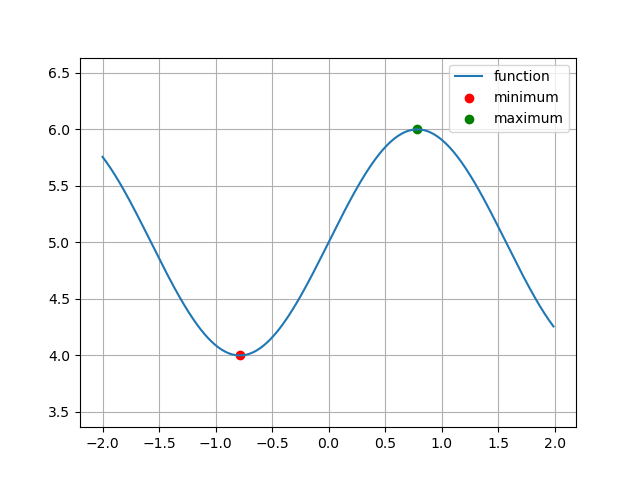
\includegraphics[width=\columnwidth]{figs/plot.png}
    \caption{Plot of local maximum and minimum}
    \label{fig:Plot1}
    \end{figure}
\end{document}}
